%!TEX root = main.tex
\problem{3}

\paragraph{Encoding the problem statement in terms of assignment problems}

Let $N$ be the set of all devices.

Let $(x, y)$ with $ x, y \in N$ be backup pairs where device $x$ is backed up by device $y$. It follows that that two devices can form a backup pair only if they are in distance of each other, $d[x, y] \leq D$.

Let $S$ be a valid backup scheme. Then $S = \{(x_S, y_S) | x_S, y_S \in N \}$ where the following constraints hold:

\begin{itemize}

	\item Device $x_S$ must be backed up exactly $k$ times: $c(x_S) = k$.
	
	\item All devices must be backed up: $\bigcup_{x_S \in N} x_s = N $
	
	\item Device $y_S$ must backup at most $b$ devices: $c(y_S) \leq b$.
	
	\item Device $y_S$ can either backup device $x_S$ or not: $c(x_S, y_S) \leq 1$.

\end{itemize}

A network with a viable backup scheme has the following properties:
\begin{enumerate}
	\item In a viable backup scheme there are $|N| * k$ backups.
	
	\item For a viable backup scheme to exist, $|N| *k \leq |N| * b$. This means that $k \leq b$.
	
	\item For a viable backup scheme to exist, each device $x$ must be in distance of at least $k$ other devices. This means that at least $|N| * k$ pairs of devices are in distance of each other.
\end{enumerate}

\paragraph{Solving the problem via maximum flow}

We solve the problem via maximum flow using the following algorithm:
\\

$Alg(N, d[1..n, 1..n], k, b, D):$
\begin{enumerate}

	\item Construct directed graph $G=(X \cup Y \cup \{s, t\}, E)$, $ X=Y=\{ vertice_i | \forall{n_i \in N \text{ $vertice_i$ represents $n_i$}}\}$.
	
	\item Construct edges $E = \{ x \rightarrow y \} \cup \{ s \rightarrow x \} \cup \{ y \rightarrow t \}$ such that $x \in X, y \in Y$. Edges  $x \rightarrow y$ are constructed only for devices where $d[x, y] \leq D$ and have the meaning that the device represented by vertice $x$ can be backed up by the device represented by vertex $y$ (since they are in distance of each other).
	
	\item Assign the following capacities:
	\begin{itemize}
	
		\item $C(s \rightarrow x) = k$
		
		\item $C(x \rightarrow y) = 1$
		
		\item $C(y \rightarrow t) = b$
	
	\end{itemize}
	
	Figure \ref{fig:graph} shows the graph obtained up to this point.
	
	\item Compute the maximum flow $f^*$.
	
	\item If $|f^*| \neq |N| * k$ report that no viable backup scheme exists.
	
	\item If ${|f^*| = |N| * k}$ report the viable backup scheme ${S = \{ (x_S, y_S), x_S, y_S \in N | f(x_S \rightarrow y_S) = 1) \}}$.

\end{enumerate}

\begin{figure}[h!]
	\centering
		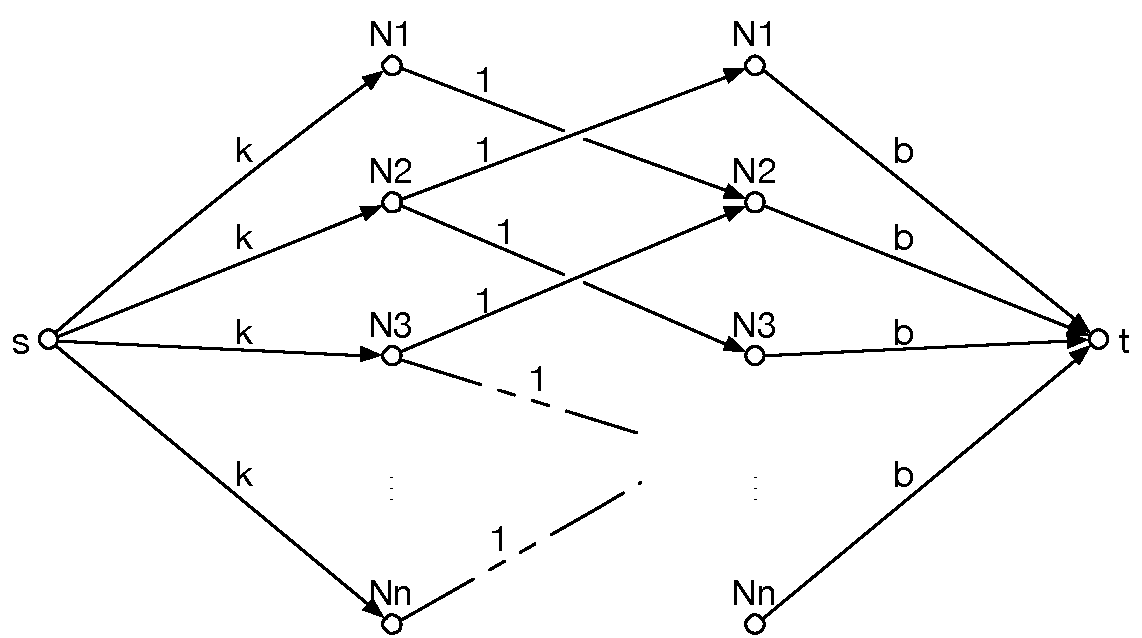
\includegraphics[width=\textwidth]{problem3}
    
	\caption{The directed graph for the backup problem together with edge capacities.}
	\label{fig:graph}
\end{figure}

\paragraph{Proofs}

\paragraph{Claim:} Let $S$ be a backup scheme for a network with the properties of a viable backup scheme. $\exists{\text{ flow } f}$ such that $|f| = |S|$.

\paragraph{Proof:} Algorithm \ref{alg:flow_constr} shows how to obtain a flow for a given backup scheme $S$. The flow maintains the conservation constraint by definition of the backup scheme: each backed up device vertex $x$ has $k$ incoming flow and an outgoing flow equal to the number of times it is backed up, which is $k$. Each backing up device $y$ has the incoming and outgoing flow equal to the number of times it is backing up other devices.


\begin{algorithm}[H]
	\caption{Flow construction for a backup scheme S}
	\label{alg:flow_constr}
	\begin{algorithmic}
	  	\For{$(x_S, y_S) \in S$}
	  		\State $f(x_S \rightarrow y_S) = 1$
	  	\EndFor
	  	
	  	\For{$x_s \in (x_S, y_S) \text{ pairs}$}
	  		\State $f(s \rightarrow x_S) = k$
	  	\EndFor
	  	
	  	\For{$y_s \in (x_S, y_S) \text{ pairs}$}
	  		\State $f(y_S \rightarrow t) = \text{number of times $y_S$ appears in S}$
		\EndFor
	\end{algorithmic}
\end{algorithm}

\paragraph{Claim:} Flow $f$ is feasible.
\paragraph{Proof:} All $s \rightarrow x_S$ edges are saturated with a flow of $k$. All $x_S \rightarrow y_S$ edges have a flow of either 1 or 0. All $y_S \rightarrow t$ edges have a flow of at most $b$ since a device can back up at most $b$ other devices.

\paragraph{Claim:} Flow $f$ is maximal with $|f| = |N| * k$.
\paragraph{Proof:} All $s \rightarrow x_S$ edges are saturated with a flow of $k$. There are $|N|$ such edges. There can be no bigger flow than the one that saturates all the outgoing edges from the source.

\paragraph{Claim:} Let $f$ be a maximal flow in the directed graph $G$ computed by algorithm \ref{alg:flow_constr} that follows the constraints for a viable backup scheme. $\exists{ \text{ backup scheme } S}$ for $f$.
\paragraph{Proof:} 
\begin{enumerate}
	\item $f$ either saturates $x \rightarrow y$ edges or avoids them.
	
	\item For each vertice $x$ there are $k$ $x \rightarrow y$ edges. This is because the maximum flow $|f| = |N| * k$ saturates all $s \rightarrow x$ edges which forces the outgoing flow of all $x$ vertices to be $k$. 
	
	\item Each $y$ vertice has an incoming flow of at most $b$. This constraint is imposed by the only outgoing edge from $y$, which is $y \rightarrow t$ of capacity $b$. 
	
	\item From the previous points we can pick $S$ as the backup scheme represented by the $x \rightarrow y$ edges that have a flow of 1. Each $x$ vertice transports a flow of $k$ which means that devices represented by $x$ are backed up exactly $k$ times. Each $y$ vertice transports a flow of at most $b$ which means that devices represented by $y$ back up at most $b$ other devices.
\end{enumerate}




